%%%%%%%%%%%%%%%%%%%%%%%%%%%%%%%%%%%%%%%%%%%%%%%%%%%%%%%%%%%%%%%%%%%
% Background
% Year:
% 2016、2017
% Team:
% Wolverine、RCPL
% Members: 
% Dexter Chen(Wolverine/2016), Eric Chang(Wolverine/2016), Eric Lee(Wolverine/2016), 
% Jacky Wu(Wolverine/2016), Karthick Mani(Wolverine/2016), Kenvin Lo(Wolverine/2016), 
% Yu-cheng Chen(Wolverine/2016), Paul Lin(RCPL/2017)
% (Format:Name(Team/Year))
% Relative files:
% Main.tex, Background_Information_retrieval_on_existing_database.tex, Library.bib, Wolverine_Background_Chart_1.png
% Note: 
% Do not compile this file compile Main.tex to get the pdf file instead.
%%%%%%%%%%%%%%%%%%%%%%%%%%%%%%%%%%%%%%%%%%%%%%%%%%%%%%%%%%%%%%%%%%%
	
\subsection{Information retrieval on existing database}
	We live in the time when technology develops rapidly. Information grows in an exponential rate. Tague1981 forecasted the further into the future we go, the fewer the additional number of first-rate publications. The information develops from linear growth to exponential growth. Thus we can't rely on the old ways to find the information we need. We need new information retrieval methods to handle the big amount of data systematically. Howeverm, most of the information retrieval methods such as search engine can not search everything on the web. 
	Grehan2002 claimed a search engine which can only search the subset of the web it has ‘captured’ and included in its own database. Thus, we need to create a database to store these data and automatically update them.
	There are several online libraries currently available for us to get the academic articles or periodicals we need.
	Besides, they can be roughly divided into three groups according to the way they store articles based on the division used by National Taiwan University Library.

\paragraph{Index libraries}
	These kind of libraries store the index and abstract of the articles.
	They don't provide the full-text documents directly, but they may give the linkage to the publisher websites of articles.
	Besides, they can be categorized by the type of articles they include.
	
	\begin{itemize}		
		\item\textbf{Comprehensive topics}\\Libraries such as Web of Science, Scopus, Google Scholar...
		\item\textbf{Specialized topics}\\Libraries such as Compendex, BIOSIS Previews, PubMed, MEDline...		
	\end{itemize}
	
\paragraph{Publisher libraries}
	These libraries are created by the publishers themselves, so they provide the newest and complete the documents directly.
	Besides, they can also be categorize by the type of articles they include.
	
	\begin{itemize}		
		\item\textbf{Comprehensive topics}\\Libraries such as Science Direct, Springer Link, Wiley Online Library...
		\item\textbf{Specialized topics}\\Libraries such as Nature.com, Emerald Management Xtra, IEEE Xplore...	
	\end{itemize}
	
\paragraph{Aggregator libraries}
	These libraries do not publish the articles by themselves, but they still sometimes provide the user with the full-text articles.
	The way they do this is to negotiate with some of the publisher libraries and get the authorization of the articles.
	Libraries such as EBSCOhost, ProQuest, JSTOR...

	The comparison between these libraries can be found on Figure \ref{WBC1}.
	On the next section we will discuss about more details about some of the existing libraries.

\begin{figure*}[htb]
	\begin{center}
		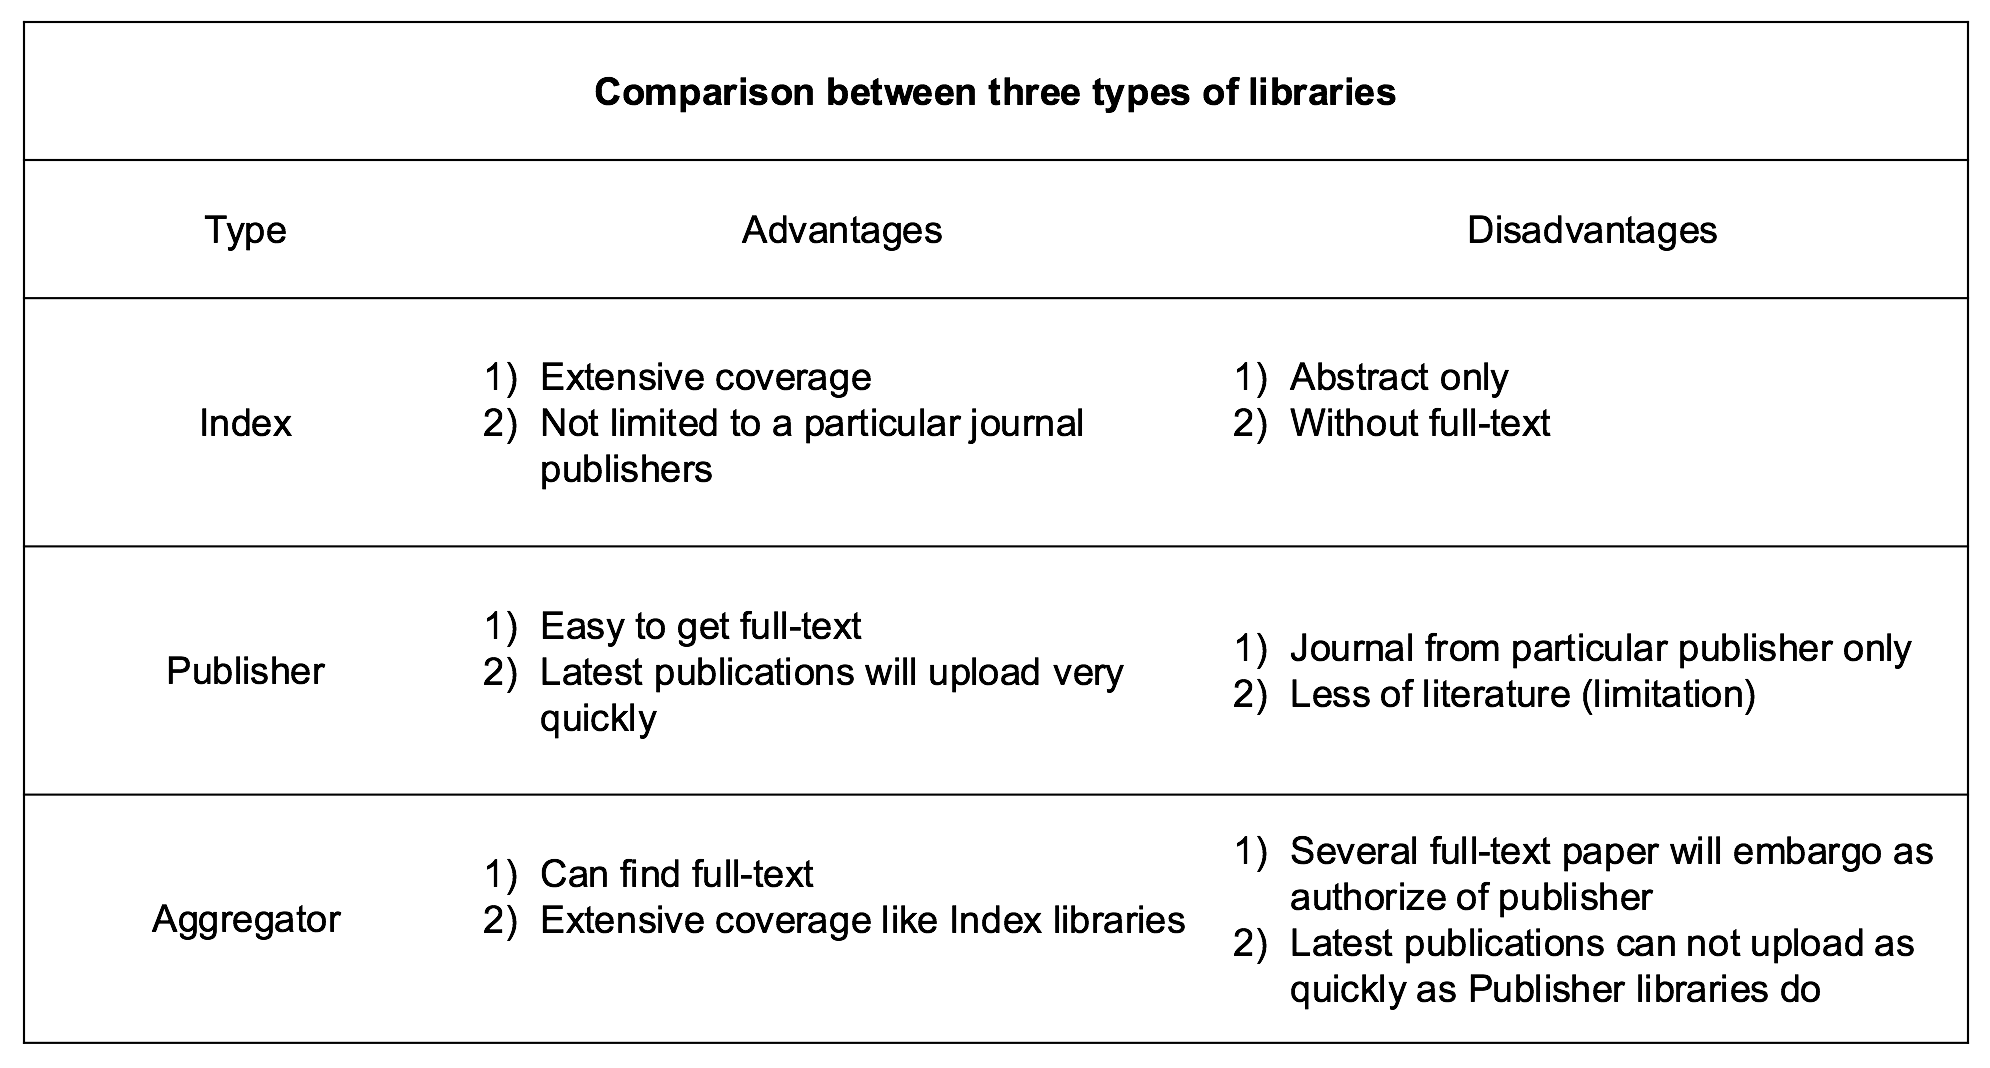
\includegraphics[width=0.8\textwidth]{Wolverine_Background_Chart_1}
	\end{center}
	\caption{Comparison between three types of libraries.\label{WBC1}}
\end{figure*}
\newpage

\subsubsection{Introduction to libraries }

\begin{enumerate}
	
	\item\textbf{PubMed}
	\setlength{\parindent}{1em}
	 PMC (PubMed Central) was launched in 2000.
	 PubMed citations often include links to the full-text article on the publishers' web sites or in PMC and the Bookshelf.
	 PubMed is a free library which is used for searching reference papers and abstracts related to the biomedical topics.
	 The largest subset of PubMed is MEDLINE, which is a bibliographic database containing life sciences and biomedical information.
	 Both of them are built by National Library of Medicine. You may limit your search to MEDLINE only in PubMed.
	 A strong feature of PubMed is its ability to link MeSH(Medical Subject Headings) terms automatically. 
	 It is useful for people who want to find the medical articles. 
     Simple searches on PubMed can be carried out by entering the key words of a subject into PubMed's search window.
     PubMed translates this initial search formulation and automatically adds field names.
	 Like several libraries, people can find the specific result they desire by adding relevant MeSH terms, synonyms and Boolean operators.	 
	 The design philosophy of PubMed is based on full-text XML files, which are readable by machines, humans and moreover technology independent.
	 PubMed is classified into Index libraries, which is the prime reason that it is not able to provide full text for some papers.
	 The type of database used by PubMed is Microsoft SQL server, which is a relational database to store all of the archives such as XML, images, and PDF files supplementary.
	
	\item\textbf{IEEE Xplore}
	\setlength{\parindent}{1em}	
	IEEE is an acronym for Institute of Electrical and Electronics Engineers, which is one of the leading standard organizations in the world. 
	Besides, it is one of the world's largest technical professional organization dedicated to advancing technology for the benefit of humanity. 
	There are more than 420,000 IEEE members in over 160 countries.
	And IEEE Xplore is a scholarly research library formerly known as IEEE/IET Electronic Library (IEL).
	The articles covered by IEEE Xplore are mainly from the IEEE and the Institution of Engineering and Technology(IET).
	More than 3.5-million full-text documents are in the field of electrical, engineering, computer science, and electronics are provided in this library. 
	There are many features in IEEE. It can rank the articles according to their click through rates or download times. 
    If some articles are updated by an author, those who set research alert on it will receive a notification through email by IEEE.
    However, some of the features are available for members only.
    Many enterprises and schools are the members of IEEE.
    
	The front and user interface of IEEE library present the information on the screen, including the latest Angular, Jquery, HTML 5, CSS.
	Most of the HTML for PDF,  it is not only for journal (conference) articles but also for standards get dynamic transformations in real time and served through MarkLogic.
	Endeca, which is an Oracle product powers Xplore searches, is used in the search layer.
	All PDF files are fed through Endeca system.
	Endeca servers will provide the matching documents and Xplore platform will present it on the screen to the user.
	Beside, all contents are stored in oracle metadata which will be consumed by Endeca, MarkLogic Authentication, and Authorization services.
	
	\item\textbf{EBSCOhost}
	\setlength{\parindent}{1em}

	EBSCOhost is a popular reference which authorizes users to gain a great many full-text articles from proprietary databases.
	EBSCO Information Services, headquartered in Ipswich, Massachusetts, which is a division of EBSCO Industries Inc., the third largest private company in Birmingham, Alabama with annual sales of nearly $2$ billion according to the BBJ's 2013 Book of Lists.
    EBSCO offers library resources to customers in academic, medical, K–12, public library, law, corporate, and government markets. 
	Its products include EBSCONET, a complete e-resource management system, and EBSCOhost, which supplies a fee-based online research service with 375 full-text databases, a collectionof 600,000-plus ebooks, subject indexes, point-of-care medical references, and an array of historical digital archives.

    In 2010, EBSCO introduced its EBSCO Discovery Service (EDS) to institutions, which allows people to search a portfolio of journals and magazines

	\item\textbf{Google Scholar}
	\setlength{\parindent}{1em}
	
	Google Scholar is a freely accessible web search engine that indexes the full text or metadata of scholarly literature across an array of publishing formats and disciplines. Released in beta in November 2004, the Google Scholar index includes most peer-reviewed online academic journals and books, conference papers, theses and dissertations, preprints, abstracts, technical reports, and other scholarly literature, including court opinions and patents. While Google does not publish the size of Google Scholar's database, third-party researchers estimated it to contain roughly 160 million documents as of May 2014 and an earlier statistical estimate published in PLOS ONE using a Mark and recapture method estimated approximately $80-90$ coverage of all articles published in English with an estimate of 100 million. This estimate also determined how many documents were freely available on the web.
	
	Google Scholar is similar in function to the freely available CiteSeerX and getCITED. It also resembles the subscription-based tools, Elsevier's Scopus and Thomson Reuters' Web of Science.
	
	Google Scholar allows users to search for digital or physical copies of articles, whether online or in libraries. "Scholarly" searches will appear using the references from "full-text journal articles, technical reports, preprints, theses, books, and other documents, including selected Web pages that are deemed to be "scholarly." Because most of Google Scholar's search results link directly to commercial journal articles, a majority of the time users will only be able to access a brief summary of the articles topics, as well as small amounts of important information regarding the article, and possibly have to pay a fee to access the entire article. The most relevant results for the searched keywords will be listed first, in order of the author's ranking, the number of references that are linked to it and their relevance to other scholarly literature, and the ranking of the publication that the journal appears in.
	
	Using its "group of" feature, it shows the available links to journal articles. In the 2005 version, this feature provided a link to both subscription-access versions of an article and to free full-text versions of articles; for most of 2006, it provided links to only the publishers' versions. Since December 2006, it has provided links to both published versions and major open access repositories, but it still does not cover those posted on individual faculty web pages; access to such self-archived non-subscription versions is now provided by a link to Google, where one can find such open access articles.
	
	Through its "cited by" feature, Google Scholar provides access to abstracts of articles that have cited the article being viewed. It is this feature in particular that provides the citation indexing previously only found in CiteSeer, Scopus and Web of Science. Through its "Related articles" feature, Google Scholar presents a list of closely related articles, ranked primarily by how similar these articles are to the original result, but also taking into account the relevance of each paper.
	
	At December 2009, Google Scholar is not yet available to the Google AJAX API.\\
	
	Google Scholar's legal database of US cases is extensive. Users can search and read published opinions of US state appellate and supreme court cases since 1950, US federal district, appellate, tax and bankruptcy courts since 1923 and US Supreme Court cases since 1791. Google Scholar embeds clickable citation links within the case and the How Cited tab allows lawyers to research prior case law and the subsequent citations to the court decision.The Google Scholar Legal Content Star Paginator extension inserts Westlaw and LexisNexis style page numbers in line with the text of the case.\\
	
	While most academic databases and search engines allow users to select one factor (e.g. relevance, citation counts, or publication date) to rank results, Google Scholar ranks results with a combined ranking algorithm in a "way researchers do, weighing the full text of each article, the author, the publication in which the article appears, and how often the piece has been cited in other scholarly literature". Research has shown that Google Scholar puts high weight especially on citation counts and words included in a document's title. As a consequence, the first search results are often highly cited articles.\\
		
	Limitations and criticism
	Quality — Some searchers consider Google Scholar of comparable quality and utility to commercial databases.The reviews recognize that its "cited by" feature in particular poses serious competition to Scopus and Web of Science. An early study, from 2007, limited to the biomedical field, found citation information in Google Scholar to be "sometimes inadequate, and less often updated". The coverage of Google Scholar may vary by discipline compared to other general databases.
	
	Coverage — Especially early on, some publishers did not allow Scholar to crawl their journals. Elsevier journals have been included since mid-2007, when Elsevier began to make most of its ScienceDirect content available to Google Scholar and Google's web search. As of February 2008 the absentees still included the most recent years of the American Chemical Society journals. Google Scholar does not publish a list of scientific journals crawled, and the frequency of its updates is unknown. It is therefore impossible to know how current or exhaustive searches are in Google Scholar, although a recent study estimates that Google Scholar can find almost $90$ (approximately 100 million) of all scholarly documents on the Web written in English. Nonetheless, it allows easy access to published articles without the difficulties encountered in some of the most expensive commercial databases.
	
	Matthew effect — Google Scholar puts high weight on citation counts in its ranking algorithm and therefore is being criticised for strengthening the Matthew effect; as highly cited papers appear in top positions they gain more citations while new papers hardly appear in top positions and therefore get less attention by the users of Google Scholar and hence fewer citations.
	
	Google Scholar effect – It is a phenomenon when some researchers pick and cite works appearing in the top results on Google Scholar regardless of their contribution to the citing publication because they automatically assume these works’ credibility and believe that editors, reviewers, and readers expect to see these citations.
	
	Incorrect field detection — Google Scholar has problems identifying publications on the arXiv preprint server correctly. Interpunctuation characters in titles produce wrong search results, and authors are assigned to wrong papers, which leads to erroneous additional search results. Some search results are even given without any comprehensible reason.
	
	Vulnerability to spam — Google Scholar is vulnerable to spam. Researchers from the University of California, Berkeley and Otto-von-Guericke University Magdeburg demonstrated that citation counts on Google Scholar can be manipulated and complete non-sense articles created with SCIgen were indexed from Google Scholar. They concluded that citation counts from Google Scholar should only be used with care especially when used to calculate performance metrics such as the h-index or impact factor. Google Scholar started computing an h-index in 2012 with the advent of individual Scholar pages. Several downstream packages like Harzing's Publish or Perish also use its data. The practicality of manipulating h-index calculators by spoofing Google Scholar was demonstrated in 2010 by Cyril Labbe from Joseph Fourier University, who managed to rank "Ike Antkare" ahead of Albert Einstein by means of a large set of SCIgen-produced documents citing each other (effectively an academic link farm).
	
	Inability to shepardize case law — As of 2010, Google Scholar was not able to shepardize case law, as Lexis can.
	
	Lack of screening for quality — Google Scholar strives to include as many journals as possible, including predatory journals, which "have polluted the global scientific record with pseudo-science, a record that Google Scholar dutifully and perhaps blindly includes in its central index."\\
	
	\item\textbf{Comparison Xplore}
	\setlength{\parindent}{1em}
	
	PubMed is a free library which contains many databases, like Medline, PreMedline and Publisher Supplied Citations.
    Medline is the largest subset of PubMed.
    One can also access MEDLINE through EBSCOhost.  
    EBSCOhost promises a large number of databases. 
	Many of them, such as MEDLINE and EconLit, are licensed from web content vendors.
    Others, such as Criminal Justice Abstracts, MasterFILE, are compiled by EBSCO itself.

    However, in contrast to other two libraries, the advanced search of PubMed is weak. 
    It does not show citation times or further information.
    And the only database which does not provide full-text documents is PubMed. 

    The documents in PubMed are almost related to the biomedical topics.
    IEEE contains more than one third documents in the field of electrical, engineering, computer science and electronics.
    And the articles in EBSCOhost comprises many fields, like business, education, laws, medical, computer science, and so on.

    Each library has its own features. PubMed can link the MeSH. EBSCOhost can be searched for the videos or photos concerned with the key words you enter. 
    IEEE has many features the other two databases don’t have, like “top downloads list”, “top search terms” and “custom setting” mentioned above.

    

\end{enumerate}

\todo[inline]{You need to add at least one library example of each library type, since you started with different types. Otherwise you could have focused on one type and motivated the focus. For the libraries containing articles you should add several since you are building one. You should also discuss the database techniques, including alternative ones to the used ones, such as MongoDB, Hadoop, etc. Try to compare features.}